\documentclass{article}
\usepackage{scribe}
\usepackage{epsfig}
\usepackage{amsmath}
\renewcommand{\Pr}[1]{\textrm{\textup{Pr}}\left( #1 \right)}
\newenvironment{slist}
  {\begin{list}{$\bullet$}{\parsep0pt\itemsep0pt\topsep0pt}}
  {\end{list}}

\title{Polynomial-Time Approximation Algorithms\\ 6.854 Scribe Notes \#20}
\date{October 27, 2006}
\author{Lecturer: David Karger\\ Scribes: Matt Doherty, John Nham, Sergiy Sidenko, David Schultz}

\begin{document}

%%%%%%%%%%%%%%%%%%%%%%%%%%%%%%%%%%%%%%%%%%%%%%%%%%%%%%%%%%%%%%%%%%%%%%
% Your notes start here!
%%%%%%%%%%%%%%%%%%%%%%%%%%%%%%%%%%%%%%%%%%%%%%%%%%%%%%%%%%%%%%%%%%%%%%
%
% For theorems, lemmas, definitions, remarks, etc. use commands
% {\theorem{...}}, {\lemma{...}}, {\definition{...}}, etc.
% For proofs, use \begin{proof} ... \end{proof}
%
% For postscript figures (.ps) use the following block:
%
% \begin{figure}[h]
% \begin{center}
% \mbox{\psfig{figure=notes-nn-fig-mm.ps}}
% \caption{A very nice picture.}
% \label{fig:picture}
% \end{center}
% \end{figure}
%

% For encapsulated postscript figures (.eps) use the following block:
%  (also change documentstyle line )
% \begin{figure}[h]
% \begin{center}
% \mbox{\epsfbox{notes-nn-fig-mm.eps}}
% \caption{A very nice picture.}
% \label{fig:picture}
% \end{center}
% \end{figure}
%


%%%%%%%%%%%%%%%%%%%%%%%%%%%%%%%%%%%%%%%%%%%%%%%%%%%%%%%%%%%%%%%%%%%%%%

$NP$-hard problems are a vast family of problems that, to the best of
our knowledge, cannot be solved in polynomial time.\footnote{Briefly, $P$ is the set of problems solvable in
  polynomial time, and $NP$ is a particular superset of $P$.  A
  problem is $NP$-hard if it is at least as hard as all problems in
  $NP$, and $NP$-complete if it is in $NP$ and it is also $NP$-hard.
  An unproven but generally accepted conjecture, which we will assume
  is true, is that $P\ne NP$.}  When presented with a $NP$-hard problem, we can take one of three possible strategies:

\begin{itemize}
\item Run a super-polynomial algorithm anyway.  Techniques such as
branch-and-bound (known as $A^*$ search in the AI world) allow us to
enumerate options in a way such that we can ignore most of the problem
space.  However, the desired complexity bounds of these algorithms are
usually not provable, and even ``slightly'' super-polynomial
is often too much to be practical.
\item
Assume that the input is random, and find an algorithm that will perform well in the average case. For example, the maximum clique problem, which is $NP$-hard, can actually be solved efficiently assuming a random input because the maximum clique in a randomly chosen graph is small. This assumption is often used in practice, but the problem is that not everyone will agree on whether the input distribution is random.
\item Settle for a suboptimal solution (an approximation) that can be
found in polynomial time, and prove that this solution is ``good
enough''.  This is the technique that we will look at in the rest of
the lecture.
\end{itemize}

\section{Preliminaries}

\textbf{Definition}:
  An \textbf{optimization
  problem} consists of:
  \begin{enumerate}
    \item A set of instances $I$
    \item A set of solutions $S(I)$
    \item An objective function\footnote{The
  restriction that the range of the objective function is
  {\boldmath$R$} might be limiting in some situations, but most problems
  can be formulated this way.}
    $f: S(I)\to \mathbb{R}$
  \end{enumerate}
  The problem is to find $s\in S(I)$ that maximizes (or minimizes)
  $f(s)$.

  \emph{Example}:
  \begin{quote}
  \textbf{Graph Coloring} is an optimization problem
  with the following form:
  \begin{enumerate}
    \item $I$: graphs
    \item $S(I)$: assignments of colors to each vertex such that
                  no neighbors have the same color
    \item $f(s)$: number of colors used in $s$
  \end{enumerate}
  Thus, given a graph, we want to find the minimum number of colors we can use to color the vertices such that no two adjacent vertices have the same color.
  \end{quote}

Some technicalities: When analyzing the complexity of optimization problems, we will assume that all inputs and ranges of $f$ are rational numbers. We will also assume that if $\sigma$ is an optimal solution, then $f(\sigma)$ is polynomial in the number of bits in the input. Our goal will be to find algorithms that have a runtime polynomial in the representation of the input in bits.

Often, when people refer to $NP$-hard problems, they are referring to
decision problems, which are algorithms for which the output is
\texttt{yes} or \texttt{no}.  For example, a decision version of
the Graph Coloring problem is determining whether or not a graph is
3-colorable.  We need a notion of $NP$-hardness that applies to
optimization problems as well.

\textbf{Definition}
(\emph{NP-hardness}):
An optimization
  problem is $NP$-hard if it can be used as a subroutine to solve an
  $NP$-hard decision problem in polynomial time, with the optimization
  problem used as a black box.

\textbf{Definition}:
An \textbf{approximation algorithm} is \textit{any}
  algorithm that gives a feasible solution to an optimization problem.

The above definition of an approximation algorithm gives no measure of how good the algorithm actually is.  For instance, a valid approximation algorithm for the Graph Coloring problem is to color each vertex with its own color.  Thus, we need a way to differentiate approximation algorithms based on how ``good'' they actually are. In the rest of this lecture, we discuss two ways to measure the ``goodness'' of an algorithm by comparing its output to the optimal solution.

\section{Absolute Approximations}

One way to compare the output of an approximation algorithm to the optimal solution is to take the absolute difference between them. If we can bound this difference to a constant for any input, then we have an absolute approximation algoirthm.

\textbf{Definition}:
  $A$ is a \textbf{{\boldmath$k$}-absolute
    approximation algorithm} if $|A(I) - OPT(I)| \le k$.

The absolute value in the above definition allows us to cover both
maximization and minimization problems with the same definition - $A(I) \le OPT(I)$ in a maximization problem, and $A(I)\ge OPT(I)$ in a
minimization problem.

Our next example will involve planar graphs.  Recall the following
definition:

\textbf{Definition}:
  A \textbf{planar graph} is a graph that can be
  drawn on the blackboard without any edges crossing.

\textbf{Figure 1}. Examples of graphs that are planar:
\begin{tabular}{cc}
  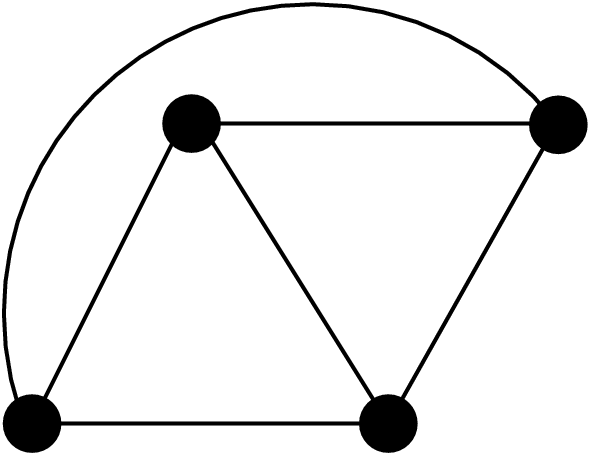
\includegraphics{approx-1.png}
  &
  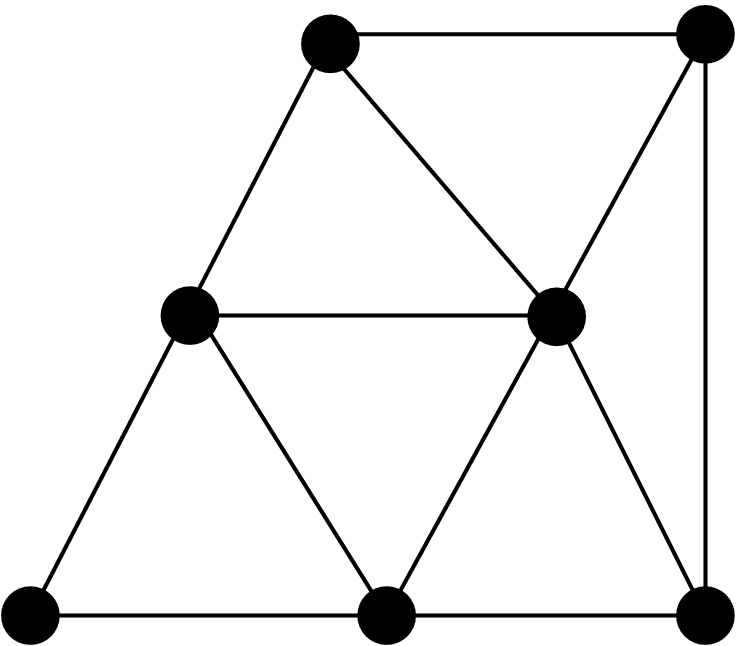
\includegraphics{approx-2.png}
\end{tabular}

\textbf{Figure 2}. Example of a graph that is \textbf{not} planar:
\begin{tabular}{c}
  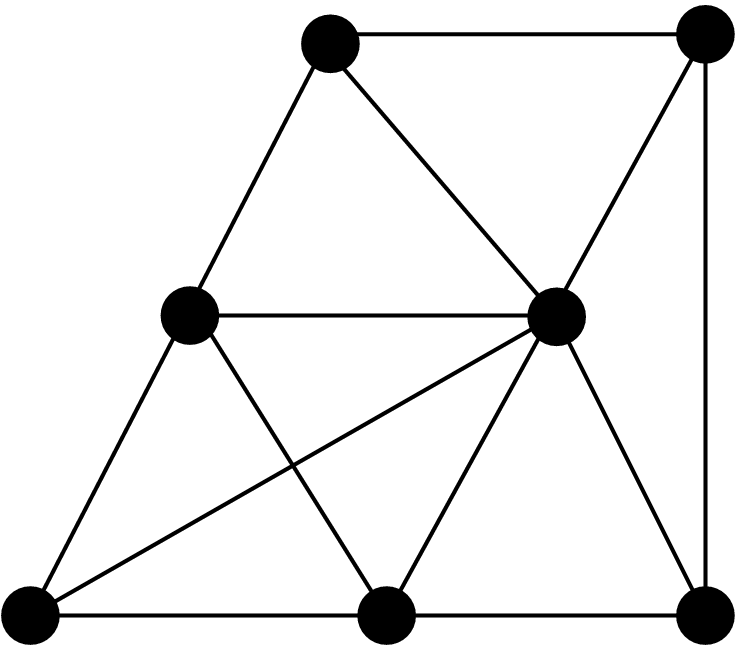
\includegraphics[width=0.5\textwidth]{approx-3.png}
\end{tabular}

Euler's formula for planar graphs tells us that $m \le 3n-6$ for $n\ge
3$, where $n$ is the number of vertices and $m$ is the number of
edges.  As a particular corollary, every planar graph has at least one
vertex with degree less than 6, since the sum of the degrees of the
vertices is $2m$, which by Euler's formula is less than $6n$.


\textbf{Definition}:
  \textbf{Planar Graph Coloring} is a restricted version
  of Graph Coloring where the inputs are constrained to be planar.

\textbf{Theorem}:
There exists a 1-absolute approximation algorithm for Planar Graph
Coloring.

\begin{proof}
We will exhibit such an algorithm.  First, note that if a graph is
1-colorable, then it has no edges and we can trivially color it.
Similarly, a 2-colorable graph is bipartite, and all other graphs
require at least 3 colors.  We can color any other planar graph with 4
colors by the famous Four Color Theorem.

The complete algorithm for an arbitrary planar graph thus works as follows:
\begin{enumerate}
\item If the graph is 1-colorable, then color it optimally.
\item If the graph is bipartite, color it with 2 colors.
\item Otherwise, the graph requires at least 3 colors.  Color it with
  4 colors using the Four Color Theorem.
\end{enumerate}
This algorithm achieves a 1-absolute approximation.
\end{proof}

Unfortunately, the set of $NP$-hard problems with absolute
approximations is very small.  This is because in general, we can
transform an absolute approximation into an exact solution by a
scaling technique, which would imply that $P=NP$.  Assuming that $P\ne
NP$, we can prove that no absolute approximation exists for problems
that have this property.  We will do this for Knapsack, one of the
first problems that was shown to be $NP$-complete, and for Maximum
Independent Set, another $NP$-complete problem.

\textbf{Definition}:
In the \textbf{Knapsack} problem, we are given a
  knapsack of size $B$ and items $i$ with size $s_i$ and profit $p_i$.
  We can think of this as a kind of shoplifting problem; the goal is
  to find the subset of the items with maximum total profit that fits
  into the knapsack.

\textbf{Theorem}:
  There is no $k$-absolute approximation algorithm for
  Knapsack for any number $k$.

\begin{proof}
Suppose for the sake of contradiction that we have a $k$-absolute
approximation algorithm.  First we will consider the case where the
prices $p_i$ are integers.  We multiply all the prices by $k+1$ and
run our $k$-absolute approximation algorithm on the resulting
instance.  The difference between any two solutions in the original
instance is at least 1, so the difference between any two solutions in
the scaled instance is at least $k+1$.  As a result of scaling, the
optimum solution increases by a factor of $k+1$, but our
$k$-approximate solution is within $k$ of this.  Therefore, the
approximation algorithm gives an exact solution for the scaled graph.
We divide by $k+1$ to obtain an optimal solution for the original
graph.  This would constitute a polynomial-time solution for a problem
that is believed to be super-polynomial, so we have a contradiction.

Note that if the prices are rational numbers rather than integers, we
can simply multiply all of the prices by their common denominator,
which has a polynomial number of bits.  Then the problem reduces to
the integer case above.
\end{proof}

\textbf{Definition}:
In the \textbf{Maximum Independent Set} problem, we are given a graph
$G$ and we must find the largest subset of the vertices in $G$ such
that there is no edge between any two vertices in the set.

Note that a graph's maximum independent set is identical to the
maximum clique in the complementary graph.  (The complement of a graph
is the graph obtained by taking the same set of vertices as in the
original graph, and placing edges only between vertices that had no
edges between them in the original graph.)

\textbf{Theorem}:
There is no $k$-absolute approximation for Maximum Independent Set,
for any number $k$.

\begin{proof}
Suppose for the sake of contradiction that we have a $k$-absolute
approximation algorithm for Maximum Independent Set.  Although there
are no numbers to scale up in this problem, there is still a scaling
trick we can use.

For an instance $G$, we make a new instance $G'$ out of $k+1$ copies
of $G$ that are not connected to each other.  Then a maximum
independent set in $G'$ is composed of one independent set in each
copy of $G$, and in particular, $OPT(G')$ is $k+1$ times as large as
$OPT(G)$.  A $k$-absolute approximation to a maximum independent set
of $G'$ has size at least $(k+1)|OPT(G)|-k$.  This approximation
consists of independent sets in each copy of $G$.  At least one of the
copies must contain a maximum independent set (i.e., an independent
set of size $|OPT(G)|$), because otherwise the total number of
elements in the approximation would be at most $(k+1)|OPT(G)| -
(k+1)$, contradicting the assumption that we have a $k$-absolute
approximation.  Hence, we can obtain an exact solution to Maximum
Independent Set in polynomial time, which we presume is impossible.
\end{proof}

\section{Relative Approximation Algorithms}

Since \textit{absolute} approximations are often not achievable, we
need a new technique---a new way to measure approximations.  Since
we can't handle additive factors, we will try multiplicative ones.

\textbf{Definition}:
An {\boldmath$\alpha$}\textbf{-approximate solution} $S(I)$ has value
$\le \alpha|OPT(I)|$ if the problem is a minimization problem and
value $\ge |OPT(I)|/\alpha$ if the problem is a maximization problem.

\textbf{Definition}:
An algorithm has an \textbf{approximation ratio} $\alpha$ if it
always yields an $\alpha$-approximate solution.

Of course, $\alpha$ must be at least 1 in order for these definitions
to make sense.  We often call an algorithm with an approximation ratio
$\alpha$ an $\alpha$-approximate algorithm.  Since absolute
approximations are so rare, people will assume that a relative
approximation is intended when you say this.

Once we have formulated an algorithm, how can we prove that it is
$\alpha$-approximate?  In general, it is hard to describe the optimal
solution, since it is our inability to talk about $OPT$ that prevents
us from formulating an exact polynomial-time algorithm for the
problem.  Nevertheless, we can establish that an algorithm is
$\alpha$-approximate by comparing its output to some upper or lower
bound on the optimal solution.

Greedy approximation algorithms often wind up providing relative
approximations.  These greedy methods are algorithms in which we take
the best local step in each iteration and hope that we don't
accumulate too much error by the time we are finished.

% Since absolute approximation algorithms are known to exist %for so few optimization problems, a
% better class of approximation algorithms to consider are %relative approximation algorithms.
% Because they are so commonplace, we will, from now on, refer to them simply as approximation algorithms.
% 
% \begin{definition}
%   \textbf{An $\alpha$-approximation algorithm} finds a solution of value at most $\alpha \cdot
%   OPT(I)$ for a minimization problem and at least $OPT(I) / \alpha$ for a maximization problem ($\alpha \ge 1$).
% \end{definition}
% 
% Note that although $\alpha$ can vary with the size of the input, we will only consider those cases
% in which it is a constant. 

To illustrate the design and analysis of an $\alpha$-approximation algorithm,
let us consider the Parallel Machine Scheduling problem, a generic form of
load balancing.

\begin{quote}
  \textbf{Parallel Machine Scheduling}:

Given $m$ machines $m_i$ and $n$ jobs with processing times $p_j$, assign the jobs to the machines
to minimize the load

$$
\max\limits_{i} \sum\limits_{j \in i} p_j,
$$

the time required for all machines to complete their assigned jobs. In scheduling notation, this
problem is described as $\mathrm {P \parallel C_{\max}}$.
\end{quote}

A natural way to solve this problem is to use a \textit{greedy algorithm} called \textbf{list
scheduling}.

\textbf{Definition}:
A \textbf{list scheduling} algorithm assigns jobs to machines by assigning each job to the least
loaded machine.

Note that the order in which the jobs are processed is not specified.

\subsection{Analysis}

To analyze the performance of list scheduling, we must somehow compare its solution for each
instance $I$ (call this solution $A(I)$) to the optimum $OPT(I)$. But we do not know how to obtain
an analytical expression for $OPT(I)$. Nonetheless, if we can find a meaningful lower bound
$LB(I)$ for $OPT(I)$ and can prove that $A(I) \le \alpha \cdot LB(I)$ for some $\alpha$, we then
have

$$
\begin{array}{lcl}
A(I)    & \le & \alpha \cdot LB(I) \\
        & \le & \alpha \cdot OPT(I).
\end{array}
$$

Using the idea of lower-bounding $OPT(I)$, we can now determine the performance of list
scheduling.

\textbf{Claim}:
List scheduling is a $(2-1/m)$-approximation algorithm for Parallel Machine Scheduling.

\begin{proof}

Consider the following two lower bounds for the optimum load $OPT(I)$:

\begin{itemize}

\item the maximum processing time $p = \max_j p_j,$
\item the average load $L = \sum_j p_j/m.$

\end{itemize}

The maximum processing time $p$ is clearly a lower bound, as the machine to which the corresponding
job is assigned requires at least time $p$ to complete its tasks. To see that the average load is
a lower bound, note that if all of the machines could complete their assigned tasks in less than
time $L$, the maximum load would be less than the average, which is a contradiction. Now suppose
machine $m_i$ has the maximum runtime $L = c_{\max}$, and let job $j$ be the last job that was
assigned to $m_i$. At the time job $j$ was assigned, $m_i$ must have had the minimum load (call it
$L_i$), since list scheduling assigns each job to the least loaded machine. Thus,

$$
\begin{array}{lcl}
\sum\limits_{\mbox{all machine i}} p_i  & \ge & m L_i + p_j \\
                                    & = & m (L - p_j) + p_j
\end{array}
$$

Therefore,

$$
\begin{array} {lcl}
OPT(I)  & \ge & \frac{1}{m} \left( m (L - p_j) + p_j \right) \\
        & = & L - (1-1/m) p_j, \\
\mbox{so}        \\
L       & \le & OPT(I) + (1 - 1/m) p_j \\
        & \le & OPT(I) + (1 - 1/m) OPT(I) \\
        & \le & (2 - 1/m) OPT(I).
\end{array}
$$

The solution returned by list scheduling is $c_{\max}$, and thus list scheduling is a
$(2-1/m)$-approximation algorithm for Parallel Machine Scheduling.

The example with $m(m-1)$ jobs of size $1$ and one job of size $m$ for $m$ machines shows that we
cannot do better than $(2-1/m)OPT(I)$.

\end{proof}

\textbf{Definition}:
In the \textbf{Maximum Cut} problem (for undirected graphs), we are
given an undirected graph and wish to partition the vertices into two
sets such that the number of edges crossing the partition is maximized.

\emph{Example}
(\textbf{A Greedy Algorithm for Maximum Cut}):
In each step, we pick any vertex and place it on one side of the cut
or the other.  In particular, we place each vertex on the side
opposite most of its previously placed neighbors.  (If the vertex has
no previously placed neighbors, or an equal number of neighbors on
each side, then we place it on either side.)  The algorithm terminates
when all vertices have been placed.

We can say very little about the structure of the optimum solution to
Maximum Cut for an arbitrary graph, but there's an obvious bound on
the number of edges in the cut, namely $m$, the total number of edges
in the graph.  We can measure the goodness of our greedy algorithm's
approximation with respect to this bound.

\textbf{Theorem}:
The aforementioned greedy algorithm for Maximum Cut is 2-approximate.

\begin{proof}
We say that an edge is ``fixed'' if both of its endpoints have been
placed.  Every time we place a vertex, some number of edges get
fixed.  At least half of these edges are cut by virtue of the
heuristic used to choose a side for the vertex.  The algorithm
completes when all edges have been fixed, at which point $m/2$ edges
have been cut, whereas we know that optimum solution has at most $m$
edges.
\end{proof}

The approach we just described was the best known approximation
algorithm for Maximum Cut for a long time.  It was improved upon in
the last decade using a technique that we will discuss in the next
lecture.

\begin{quote}
\emph{Example}
\textbf{A Clustering Problem}: Suppose we are given a set of points,
along with distances satisfying the triangle inequality.  Our goal is
to partition the points into $k$ groups such that the maximum
\textit{diameter} of the groups is minimized.  The diameter of a group
is defined to be the maximum distance between any two points in the
group.

An approximation algorithm for this problem involves first picking $k$
cluster ``centers'' greedily.  That is, we repeatedly pick the point
at the greatest distance from the existing centers to be a new
center.  Then we assign the remaining points to the closest centers.
The analysis of this problem is left as a problem set exercise.
\end{quote}

As we demonstrated, Maximum Cut has a constant-factor approximation.
We will now consider an algorithm that has no constant-factor
approximation, i.e., $\alpha$ depends on the size of the input.

\textbf{Definition}:
In the \textbf{Set Cover} problem, we are given a collection of $n$ items
and a collection of (possibly overlapping) sets, each of which
contains some of the items.  A \textit{cover} is a collection of sets
whose union contains all of the items.  Our goal is to produce a
cover using the minimum number of sets.

A natural local step for Set Cover is to add a new set to the cover.
An obvious greedy strategy is to always choose the set that covers the
most new items.

\textbf{Theorem}:
A greedy algorithm for Set Cover that always chooses the set that
covers the most new items is $O(\log n)$-approximate.

\begin{proof}
Suppose that the optimum cover has $k$ sets.  Then at a stage where
$r$ items remain to be covered, some set covers $r/k$ of them.
Therefore, choosing the set that covers the most new points reduces
the number of uncovered points to $r-r/k = r(1-1/k)$.  If we start
with $n$ points and repeat this process $j$ times, $r\le n(1-1/k)^j$.
Since $r$ is an integer, we are done when $n(1-1/k)^j < 1$.  This
happens when $j = O(k\log n)$.  Hence, $\alpha = j/k = O(\log n)$.
\end{proof}

This result is much better than an $O(n)$-approximate solution, but
you have to wonder if we could do better with a cleverer algorithm.
People spent a long time trying to find a constant approximation.
Unfortunately, it was recently proven that $O(\log n)$ is the best
possible polynomial-time approximation.

However, we can do better for a special case of Set Cover called
Vertex Cover.  Both problems are $NP$-hard, but it turns out that the
latter does indeed have a constant factor approximation.

\textbf{Definition}:
In the \textbf{Vertex Cover} problem, we are given a graph $G$, and we
wish to find a minimal set of vertices containing at least one
endpoint of each edge.

After seeing a greedy algorithm for Set Cover, it might seem natural
to devise a scheme for Vertex Cover in which a local step consists of
picking the vertex with the highest uncovered indegree.  This does
indeed give a $O(\log n)$ approximation, but we can do better with
another heuristic.

As a starting point, imagine that instead of looking at the number of
covered edges on each vertex, we simply picked \textit{any} uncovered
edge and covered it.  Clearly one of the two endpoints for the edge is
in the optimum cover.  Unfortunately, we might get unlucky and pick
the wrong one.  Consider the graph in Figure \ref{fig:star}.  If we
chose the peripheral vertices first, our cover would contain $n-1$
vertices.

\begin{figure}[h]
  \centering
  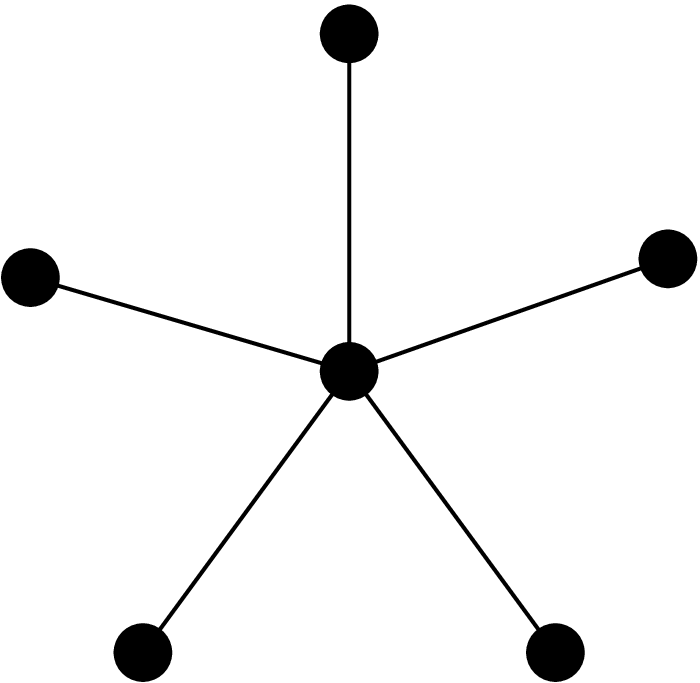
\includegraphics[width=0.6\textwidth]{approx-4.png}
  \caption{\textbf{Figure 3}. A pathological case for na\"\i ve greedy Vertex Cover.}
\label{fig:star}
\end{figure}

To solve this problem, when we choose an edge to cover, we add both of
its endpoints to the cover.  This gives us a 2-approximate cover
because one of the two endpoints is in the optimum cover.  This is a
beautiful case of bounding an approximation against a \textit{bound} of
the optimum solution without actually knowing the optimum solution.

Relatively recently, someone improved the vertex cover bound to a
$2-O(\log\log n/\log n)$ approximation with a significant amount of
work.  It is known to be impossible to do better than $4/3$, but
nobody knows how to close the gap.


\section{Polynomial Approximation Schemes}

The obvious question to ask now is how good an $\alpha$ we can obtain.

\textbf{Definition}:
A \textbf{polynomial approximation scheme (PAS)} is a set of algorithms $\{ A_\varepsilon \}$ for
which each $A_\varepsilon$ is a polynomial-time $(1+\varepsilon)$-approximation algorithm.

Thus, given any $\varepsilon >0$, a PAS provides an algorithm that achieves a
$(1+\varepsilon)$-approximation. In order to devise a PAS we can use a method called
$k$-enumeration.

\textbf{Definition}:
An approximation algorithm using \textbf{$k$-enumeration} finds an optimal solution for the $k$
most important elements in the problem and then uses an approximate polynomial-time method to
solve the reminder of the problem.

\subsection{A Polynomial Approximation Scheme for Parallel Machine Scheduling}

We can do the following:

\begin{itemize}

\item Enumerate all possible assignments of the $k$ largest jobs.

\item For each of these partial assignments, list schedule the remaining jobs.

\item Return as the solution the assignment with the minimum load.

\end{itemize}

Note that in enumerating all possible assignments of the $k$ largest jobs, the algorithm will
always find the optimal assignment for these jobs. The following claim demonstrates that this
algorithm provides us with a PAS.

\textbf{Claim}:
For any fixed $m$, $k$-enumeration yields a polynomial approximation scheme for Parallel
Machine Scheduling.

\begin{proof}

Let us consider the machine $m_i$ with maximum runtime $c_{\max}$ and the last job that $m_i$ was
assigned.

If this job is among the $k$ largest, then it is scheduled optimally, and $c_{\max}$ equals
$OPT(I)$.

If this job is not among the $k$ largest, without loss of generality we may assume that it is the
$(k+1)$th largest job with processing time $p_{k+1}$. Therefore,
$$
%\begin{array} {lcl}
A(I) \le OPT(I) + p_{k+1}.
$$
Suppose otherwise, $A(I) > OPT(I) + p_{k+1}$. Remember we must have scheduled the last job to the machine with the least load, that implies all machines had load greater than $OPT(I)$. But we argued before than $nOPT(I) \geq \Sigma p_i$, the sum of all processing times. So, before we scheduled all jobs, the total time is already larger than the sum of all the processing times, contradiction.

However, $OPT(I)$ can be bound from below in the following way:
$$
OPT(I) \ge \frac{k p_k}{m},
$$

because $\frac{k p_k}{m}$ is the minimum average load when the largest $k$ jobs have been
scheduled.

Now we have:
$$
\begin{array} {lcl}
A(I)    & \le & OPT(I) + p_{k+1} \\
        & \le & OPT(I) + OPT(I) \frac{m}{k} \\
        & = & OPT(I) \left( 1+\frac{m}{k} \right).
\end{array}
$$

Given $\varepsilon > 0$, if we let $k$ equal $m/\varepsilon$, we will get
$$
c_{\max} \le (1+\varepsilon) OPT(I).
$$

Finally, to determine the running time of the algorithm, note that because each of the $k$ largest
jobs can be assigned to any of the $m$ machines, there are $m^k = m^{m/\varepsilon}$ possible
assignments of these jobs. Since the list scheduling performed for each of these assignments takes
$O(n)$ time, the total running time is $O(nm^{m/\epsilon})$, which is polynomial because $m$ is
fixed. Thus, given an $\varepsilon >0$, the algorithm is a $(1+\varepsilon)$-approximation, and so
we have a polynomial approximation scheme.

\end{proof}

\section{Fully Polynomial Approximation Schemes}

Consider the PAS in the previous section for ${\rm P \parallel C_{\max}}$. The running time for
the algorithm is prohibitive even for moderate values of $\varepsilon$. The next level of
improvement, therefore, would be approximation algorithms that run in time polynomial in $1/
\varepsilon$, leading to the definition below.

\textbf{Definition}:
\textbf{Fully Polynomial Approximation Scheme (FPAS)} is a set of approximation algorithms such
that each algorithm $A(\varepsilon)$ in this set runs in time that is polynomial in the size of
the input, as well as in $1/ \varepsilon$.

There are few $NP$-complete problems that allow for FPAS. Below we discuss FPAS for the Knapsack
problem.

\subsection{A Fully Polynomial Approximation Scheme for the Knapsack Problem}

The Knapsack problem receives as input an instance $I$ of $n$ items with profits $p_i$, sizes
$s_i$ and knapsack size (or capacity) $B$. The output of the Knapsack problem is the subset $S$ of
items of total size at most $B$, and that has profit:

$$
\max \sum\limits_{i \in S} p_i.
$$

Suppose now that the profits are integers; then we can write a $DP$ algorithm based on the minimum
size subset with profit $p$ for items $1, \, 2, \, \ldots, \, r$ as follows:

$$
M(r,p) = \min \left\{ M(r-1,p), M(r-1, p-p_r) + s_r \right\}.
$$

The corresponding table of values can be filled in $O\left(n \sum_i p_i \right)$ (note that this
is not a FPAS in itself).

Now, we consider the general case where the profits are not assumed to be integers. Once again, we
use a rounding technique but one that can be considered a generic approach for developing FPAS for
other $NP$-complete problems that allows for FPAS. Suppose we multiplied all profits $p_i$ by
$n/(\varepsilon \cdot OPT)$; then the new optimal objective value is apparently $n/\varepsilon$.
Now, we can round the profits down to the nearest integer, and hence the optimal objective value
decreases at most by $n$; expressed differently, the decrease in objective value is at most
$\varepsilon \cdot OPT$. Using the $DP$ algorithm above, we can therefore find the optimal
solution to the rounded problem in $O(n^2/ \varepsilon)$ time, thus providing us with a FPAS in
$1/\varepsilon$.

\end{document}
